\section{1174009 - Dwi Yulianingsih}
\subsection{Teori}

\begin{enumerate}
\item Mengapa Kata-Kata Harus Di Lakukan Vektorisasi Dan Ilustrasi Gambar.
\begin{itemize}
\item Penjelasan:

Karenakan mesin hanya mampu membaca data dengan bentuk angka.Berdasarkan hal tersebut maka tentunya diperlukan vektorisasi kata atau bisa disebut dengan mengubah kata menjadi bentuk vektor agar mesin seolah-olah paham apa yang kita maksudkan dan dapat memproses aktifitas/perintah dengan benar. Selain alasan diatas, kata harus di vektorisasiuntuk mengetahui presentase kata yang sering muncul dalam setiap kalimatnya, yang berguna untuk menetukan kata kunci.

\item Ilustrasi Gambar

\begin{figure}[!hbtp]
\centering
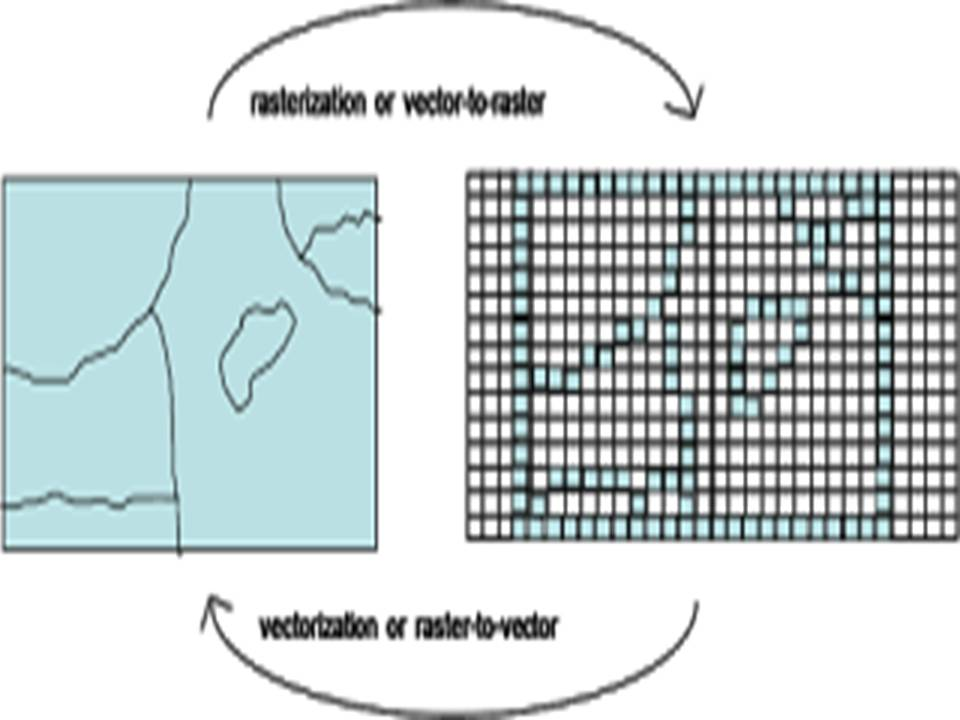
\includegraphics[scale=0.3]{figures/1174009/chapter5/5.jpg}
\caption{Vektorisasi}
\label{Vektorisasi}
\end{figure}

\end{itemize}

\break

\item Mengapa Dimensi Dari Vektor Dataset Google Bisa Mencapai 300 Dan Ilustrasi Gambar.
\begin{itemize}
\item Penjelasan:

Karena pada masing-masing objek yang terdapat pada dataset akan memiliki identitasnya tersendiri. Apabila dicontohkan dengan penjelasan yang lebih rinci maka dilakukan perumpamaan sederhana. Misalnya untuk sebuah dataset google yang memiliki 3 buah objek yaitu berat, lebar, dan tinggi.  Kemudian dari masing-masing objek tersebut dilakukan perbandingan antara berat dan lebar beserta berat dan tinggi. Hasil yang didapatkan akan memiliki presentasi yang berbeda sehingga dapat diartikan bahwa mesin dapat membedakan objek yang hampir serupa namun tak sama.

\item Ilustrasi Gambar

\begin{figure}[!hbtp]
\centering
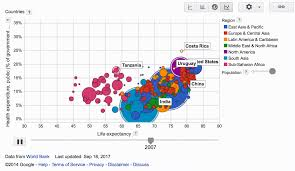
\includegraphics[scale=0.8]{figures/1174009/chapter5/7.jpg}
\caption{Dimensi Vektor Dataset}
\label{Dimensi Vektor Dataset}
\end{figure}

\end{itemize}

\break

\item Konsep Vektorisasi Untuk Kata Dan Ilustrasi Gambar.
\begin{itemize}
\item  Penjelasan:

Konsep untuk vektorisasi kata sebenarnya sama dengan ketika dilakukan input suatu kata pada mesin pencarian. Kemudian untuk hasilnya akan mengeluarkan ( berupa ) referensi mengenai kata tersebut. Jadi data kata tersebut didapatkan dari hasil pengolahan pada kalimat-kalimat sebelumnya yang telah diolah. Contoh sederhananya pada kalimat berikut ( Please click the alarm icon for more notifications about my channel ), pada kalimat tersebut terdapat konteks yakni channel, kata tersebut akan dijadikan data latih untuk mesin yang akan dipelajari dan diproses. Jadi ketika kita inputkan kta channel, maka mesin akan menampilkan keterkaitannya dengan kata tersebut sehingga akan lebih efisien dan lebih mudah.

\item Ilustrasi Gambar

\begin{figure}[!hbtp]
\centering
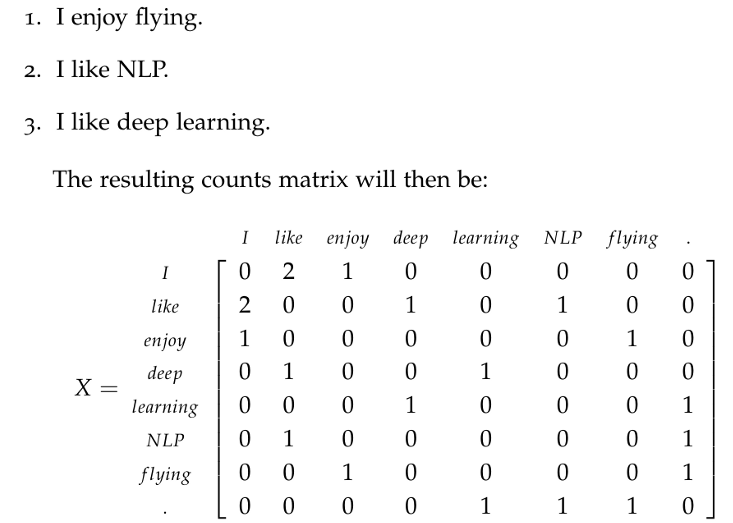
\includegraphics[scale=0.5]{figures/1174009/chapter5/4.png}
\caption{Vektorisasi Untuk Kata}
\label{Vektorisasi Untuk Kata}
\end{figure}

\end{itemize}
\break

\item Konsep Vektorisasi Untuk Dokumen Dan Ilustrasi Gambar.
\begin{itemize}
\item  Penjelasan:

Untuk vektorisasi dokumen sebenarnya terbilang sama dengan konsep vektorisasi kata, yang membedakan hanya pada proses awalnya ( pada eksekusi awal ). Untuk vektorisasi dokumen ini, mesin akan membaca semua kalimat yang terdapat pada dokumen tersebut, kemudian kalimat yang terdapat pada dokumen tersebut akan di pecah menjadi kata-kata. Seperti itulah konsep vektorisasi dokumen.

\item Ilustrasi Gambar

\begin{figure}[!hbtp]
\centering
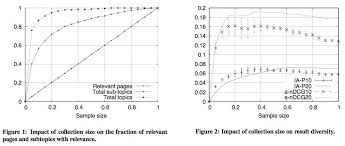
\includegraphics[scale=0.8]{figures/1174009/chapter5/6.jpg}
\caption{Vektorisasi Untuk Dokumen}
\label{Vektorisasi Untuk Dokumen}
\end{figure}

\end{itemize}
\break

\item Pengertian Mean Dan Standar Devisiasi Beserta Ilustrasi Gambar.
\begin{itemize}
\item  Pengertian Mean:

Mean adalah nilai rata-rata dari beberapa buah data. Nilai mean dapat ditentukan dengan membagi jumlah data dengan banyaknya data. Mean (rata-rata) merupakan suatu ukuran pemusatan data. Mean suatu data juga merupakan statistik karena mampu menggambarkan bahwa data tersebut berada pada kisaran mean data tersebut. Mean tidak dapat digunakan sebagai ukuran pemusatan untuk jenis data nominal dan ordinal.

\item  Pengertian Standar Devisiasi:

Standar Deviasi dan Varians Salah satu teknik statistik yg digunakan untuk menjelaskan homogenitas kelompok. Varians merupakan jumlah kuadrat semua deviasi nilai-nilai individual thd rata-rata kelompok. Sedangkan akar dari varians disebut dengan standar deviasi atau simpangan baku. Standar Deviasi dan Varians Simpangan baku merupakan variasi sebaran data. Semakin kecil nilai sebarannya berarti variasi nilai data makin sama Jika sebarannya bernilai 0, maka nilai semua datanya adalah sama. Semakin besar nilai sebarannya berarti data semakin bervariasi.

\item Ilustrasi Gambar

\begin{figure}[!hbtp]
\centering
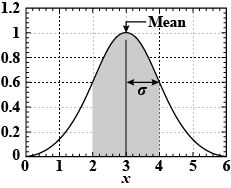
\includegraphics[scale=0.7]{figures/1174009/chapter5/2.png}
\caption{Mean}
\label{Mean}
\end{figure}

\begin{figure}[!hbtp]
\centering
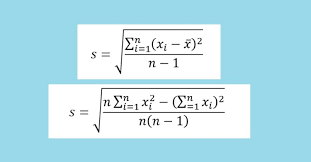
\includegraphics[scale=0.7]{figures/1174009/chapter5/3.png}
\caption{Standar Devisiasi}
\label{Standar Devisiasi}
\end{figure}

\end{itemize}

\item Penjelasan Skip-gram Dan Ilustrasi Gambar
\begin{itemize}
\item  Penjelasan:

Skip-Gram adalah kebalikannya, yaitu mencoba memprediksi vektor kata-kata yang ada di konteks diberikan vektor kata tertentu. Skip-Gram membuat sepasang kata target dan konteks sebagai sebuah instance sehingga Skip-Gram cenderung lebih baik ketika ukuran corpus sangat besar. 

\item Ilustrasi Gambar

\begin{figure}[!hbtp]
\centering
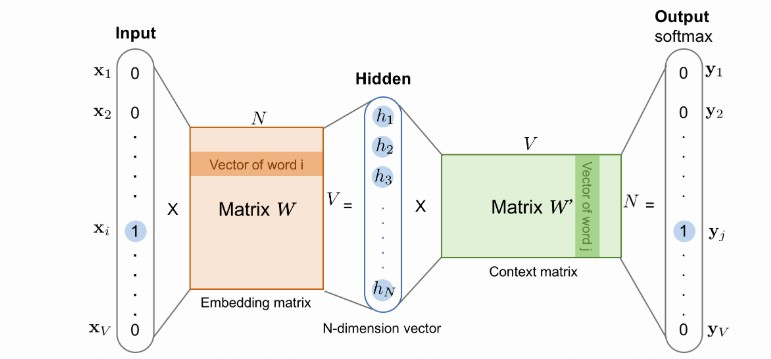
\includegraphics[scale=0.5]{figures/1174009/chapter5/1.jpg}
\caption{Skip Gram}
\label{Skip Gram}
\end{figure}
\par
\par
\end{itemize}
\par
\par
\end{enumerate}

\subsection{Praktek}
\begin{enumerate}
\item Percobaan Google Dataset ( Perbandingan Dan Similarity ) Untuk Beberapa Data Berikut :
\begin{enumerate}
\item Love

Penjelasan: Pada hasil gambar 'love' dapat dilihat bahwa nilai pada vektor baris pertamanya adalah 0.10302734. Jika dibandingkan dengan gambar 'faith' dapat dikatakan bahwa kedua gambar tersebut tidak dapat dimasukkan pada kategori yang sama.

\begin{figure}[!hbtp]
\centering
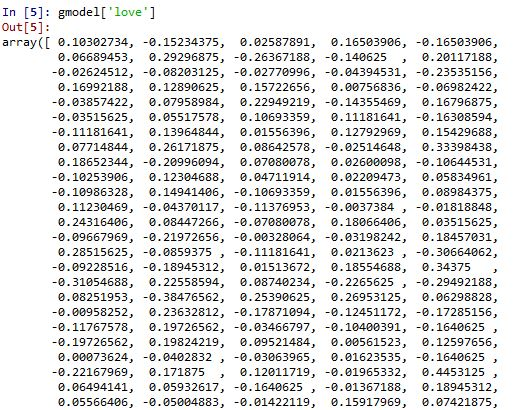
\includegraphics[scale=0.7]{figures/1174009/chapter5/12love.jpg}
\caption{Google Dataset}
\label{Google Dataset}
\end{figure}

\item Faith

Penjelasan: Pada hasil gambar 'faith' dapat dilihat bahwa nilai pada vektor baris pertamanya adalah 0.26367188. Jika dibandingkan dengan gambar 'fall' dapat dikatakan bahwa kedua gambar tersebut tidak dapat dimasukkan pada kategori yang sama.

\begin{figure}[!hbtp]
\centering
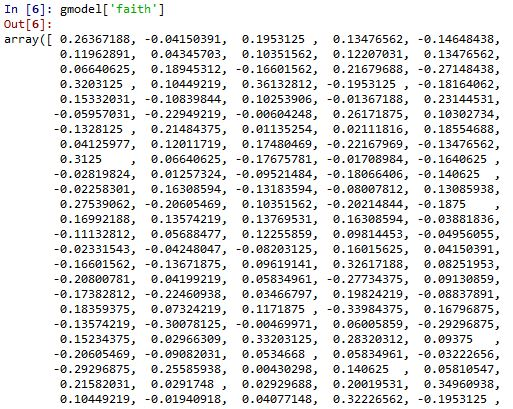
\includegraphics[scale=0.7]{figures/1174009/chapter5/13faith.jpg}
\caption{Google Dataset}
\label{Google Dataset}
\end{figure}

\item Fall

Penjelasan: Pada hasil gambar 'fall' dapat dilihat bahwa nilai pada vektor baris pertamanya adalah -0.04272461. Jika dibandingkan dengan gambar 'sick' dapat dikatakan bahwa kedua gambar tersebut tidak dapat dimasukkan pada kategori yang sama.

\begin{figure}[!hbtp]
\centering
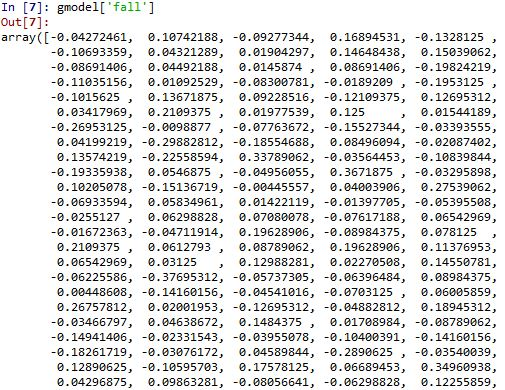
\includegraphics[scale=0.7]{figures/1174009/chapter5/14fall.jpg}
\caption{Google Dataset}
\label{Google Dataset}
\end{figure}

\item Sick

Penjelasan: Pada hasil gambar 'sick' dapat dilihat bahwa nilai pada vektor baris pertamanya adalah 1.82617188e-01. Jika dibandingkan dengan gambar 'clear' dapat dikatakan bahwa kedua gambar tersebut tidak dapat dimasukkan pada kategori yang sama.

\begin{figure}[!hbtp]
\centering
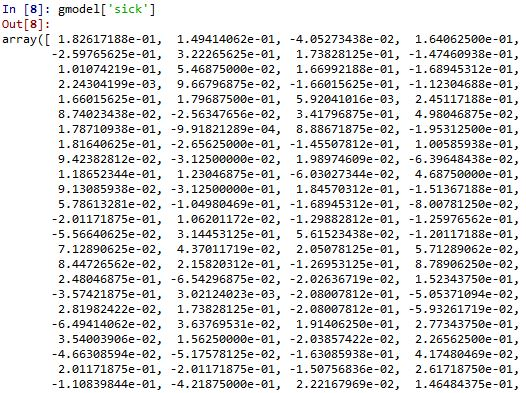
\includegraphics[scale=0.7]{figures/1174009/chapter5/15sick.jpg}
\caption{Google Dataset}
\label{Google Dataset}
\end{figure}

\item Clear

Penjelasan: Pada hasil gambar 'clear' dapat dilihat bahwa nilai pada vektor baris pertamanya adalah -2.44140625e-04. Jika dibandingkan dengan gambar 'shine' dapat dikatakan bahwa kedua gambar tersebut tidak dapat dimasukkan pada kategori yang sama.

\begin{figure}[!hbtp]
\centering
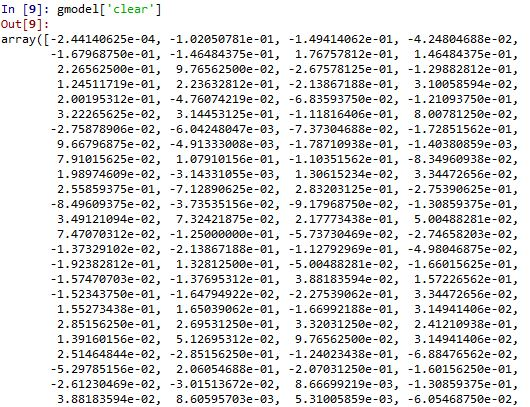
\includegraphics[scale=0.7]{figures/1174009/chapter5/16clear.jpg}
\caption{Google Dataset}
\label{Google Dataset}
\end{figure}

\item Shine

Penjelasan: Pada hasil gambar 'shine' dapat dilihat bahwa nilai pada vektor baris pertamanya adalah -0.12402344. Jika dibandingkan dengan gambar 'bag' dapat dikatakan bahwa kedua gambar tersebut tidak dapat dimasukkan pada kategori yang sama.

\begin{figure}[!hbtp]
\centering
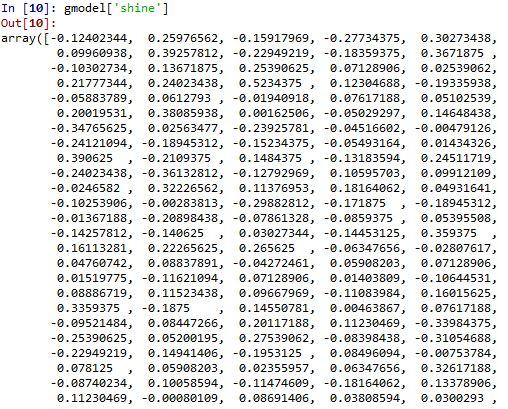
\includegraphics[scale=0.7]{figures/1174009/chapter5/17shine.jpg}
\caption{Google Dataset}
\label{Google Dataset}
\end{figure}

\item Bag

Penjelasan: Pada hasil gambar 'bag' dapat dilihat bahwa nilai pada vektor baris pertamanya adalah -0.03515625. Jika dibandingkan dengan gambar 'car' dapat dikatakan bahwa kedua gambar tersebut tidak dapat dimasukkan pada kategori yang sama.

\begin{figure}[!hbtp]
\centering
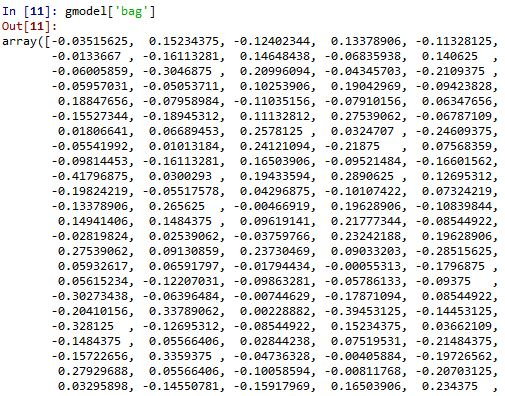
\includegraphics[scale=0.7]{figures/1174009/chapter5/18bag.jpg}
\caption{Google Dataset}
\label{Google Dataset}
\end{figure}

\item Car

Penjelasan: Pada hasil gambar 'car' dapat dilihat bahwa nilai pada vektor baris pertamanya adalah 0.13085938. Jika dibandingkan dengan gambar 'wash' dapat dikatakan bahwa kedua gambar tersebut tidak dapat dimasukkan pada kategori yang sama.

\begin{figure}[!hbtp]
\centering
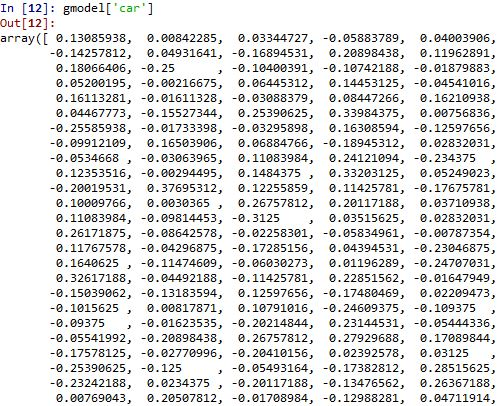
\includegraphics[scale=0.7]{figures/1174009/chapter5/19car.jpg}
\caption{Google Dataset}
\label{Google Dataset}
\end{figure}

\item Wash

Penjelasan: Pada hasil gambar 'wash' dapat dilihat bahwa nilai pada vektor baris pertamanya adalah 9.46044922e-03. Jika dibandingkan dengan gambar 'motor' dapat dikatakan bahwa kedua gambar tersebut tidak dapat dimasukkan pada kategori yang sama.

\begin{figure}[!hbtp]
\centering
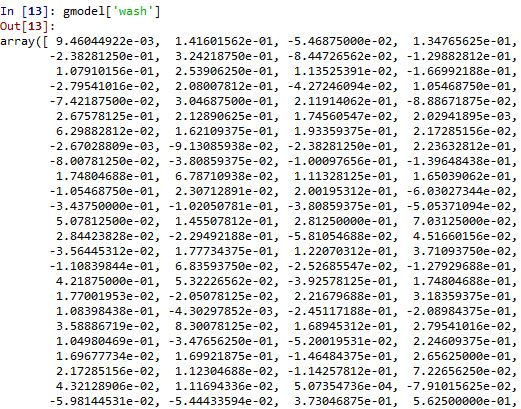
\includegraphics[scale=0.7]{figures/1174009/chapter5/20wash.jpg}
\caption{Google Dataset}
\label{Google Dataset}
\end{figure}

\item Motor

Penjelasan: Pada hasil gambar 'motor' dapat dilihat bahwa nilai pada vektor baris pertamanya adalah 5.73730469e-02. Jika dibandingkan dengan gambar 'cycle' dapat dikatakan bahwa kedua gambar tersebut tidak dapat dimasukkan pada kategori yang sama.

\begin{figure}[!hbtp]
\centering
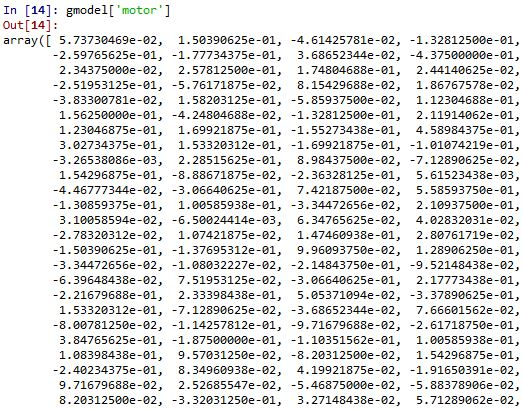
\includegraphics[scale=0.7]{figures/1174009/chapter5/21motor.jpg}
\caption{Google Dataset}
\label{Google Dataset}
\end{figure}

\item Cycle

Penjelasan: Pada hasil gambar 'cycle' dapat dilihat bahwa nilai pada vektor baris pertamanya adalah 0.04541016. Jika dibandingkan dengan gambar 'love' dapat dikatakan bahwa kedua gambar tersebut tidak dapat dimasukkan pada kategori yang sama.

\begin{figure}[!hbtp]
\centering
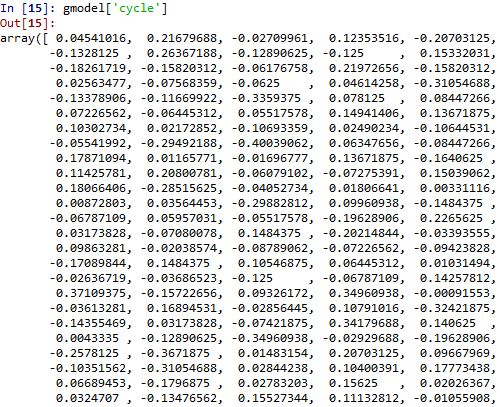
\includegraphics[scale=0.7]{figures/1174009/chapter5/22cycle.jpg}
\caption{Google Dataset}
\label{Google Dataset}
\end{figure}

\item Similarity

Penjelasan: Pada hasil gambar 'car' dapat dilihat bahwa nilai pada vektor baris pertamanya adalah 0.13085938. Jika dibandingkan dengan gambar 'love', 'sick', 'clear', 'motor', 'wash' dapat dikatakan bahwa semua gambar tersebut yang paling mendekati adalah 'sick'.

\begin{figure}[!hbtp]
\centering
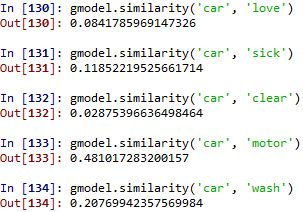
\includegraphics[scale=0.7]{figures/1174009/chapter5/23.jpg}
\caption{Google Dataset}
\label{Google Dataset}
\end{figure}

\end{enumerate}

\item Penjelasan Dan Ilustrasi ExtractWords Dan PermuteSentences
\begin{itemize}

\begin{figure}[!hbtp]
\centering
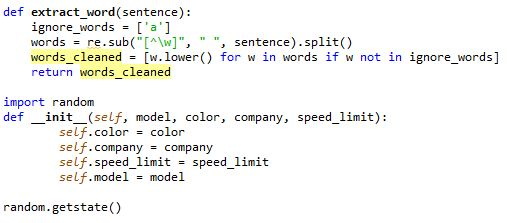
\includegraphics[scale=0.7]{figures/1174009/chapter5/32.jpg}
\caption{Extract Word dan PermuteSentence}
\label{Extract Word dan PermuteSentence}
\end{figure}

\item ExtractWords

Penjelasan:  Pada kalimat 'This isn't really a sentence' yang  akan dipisahkan perkata. Dimana library re dan library string di import terlebih dahulu. Lalu variable out mendefinisikan X untuk mengembalikan string pada objek line yang telah di split. Kemudian, X dikembalikan berdasarkan jumlah kata.

\begin{figure}[!hbtp]
\centering
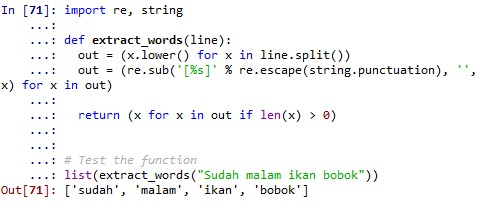
\includegraphics[scale=0.7]{figures/1174009/chapter5/29.jpeg}
\caption{ExtractWord}
\label{ExtractWord}
\end{figure}

\item PermuteSentences

Penjelasan: Digunakan untuk melakukan pengocokan atau acak pada text yang diiginkan.

\begin{figure}[!hbtp]
\centering
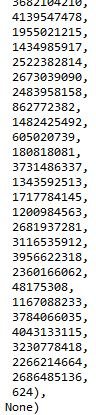
\includegraphics[scale=0.7]{figures/1174009/chapter5/31.jpg}
\caption{PermuteSentences}
\label{PermuteSentences}
\end{figure}

\end{itemize}

\item Library Gensim TaggedDocument Dan Doc2Vac
\begin{itemize}
\item Contoh atau Ilustrasi Gambar:

\begin{figure}[!hbtp]
\centering
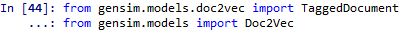
\includegraphics[scale=0.7]{figures/1174009/chapter5/40.jpg}
\caption{Tagged Document dan Doc2Vec}
\label{Tagged Document dan Doc2Vec}
\end{figure}

Penjelasan:

Import library gensim dan meng-import modul Tagged Document dan Doc2Vac.Tagged Document adalah dokumen yang 'memisahkan informasi dan struktur dari presentasi' dengan menggunakan tag. Fungsi Doc2Vec berisi alpha dan min alpha parameter, tetapi itu berarti bahwa tingkat pembelajaran meluruh selama satu periode dari alpha untuk min alpha.

\end{itemize}

\item Menambahkan Data Training (Melatih Modul Doc2Vec)
\begin{itemize}
\item Contoh atau Ilustrasi Gambar:

\begin{figure}[!hbtp]
\centering
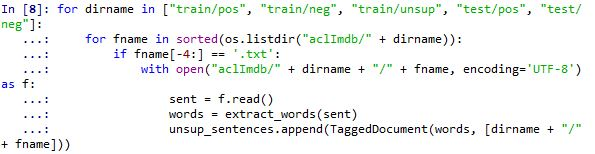
\includegraphics[scale=0.7]{figures/1174009/chapter5/42.jpg}
\caption{Model 1}
\label{Model 1}
\end{figure}

\begin{figure}[!hbtp]
\centering
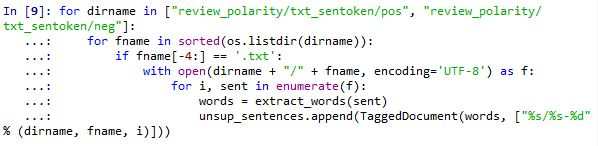
\includegraphics[scale=0.7]{figures/1174009/chapter5/43.jpg}
\caption{Model 2}
\label{Model 2}
\end{figure}

\begin{figure}[!hbtp]
\centering
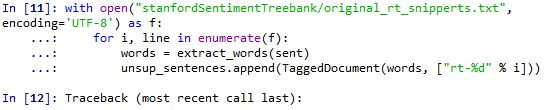
\includegraphics[scale=0.7]{figures/1174009/chapter5/44.jpg}
\caption{Model 3}
\label{Model 3}
\end{figure}

Penjelasan:

Membaca direktori name dari data yang ada di dalam kurung, terdapat ada 3 data.

\end{itemize}

\item Pengocokan Dan Pembersihan Data.
\begin{itemize}
\item Contoh atau Ilustrasi Gambar: 

\begin{figure}[!hbtp]
\centering
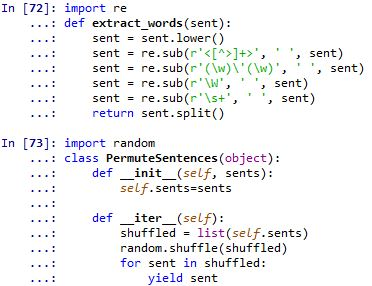
\includegraphics[scale=0.7]{figures/1174009/chapter5/60.jpg}
\caption{Pengocokan dan Pembersihan Data}
\label{Pengocokan dan Pembersihan Data}
\end{figure}

\begin{figure}[!hbtp]
\centering
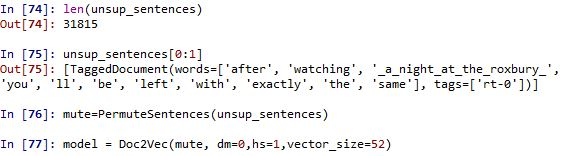
\includegraphics[scale=0.7]{figures/1174009/chapter5/61.jpg}
\caption{Pengocokan dan Pembersihan Data}
\label{Pengocokan dan Pembersihan Data}
\end{figure}

Penjelasan:

Mengimport Library Re. Kemudian membuat fungsi utuk menghapus tag html dan perkocokan. Dimana di dalam variabel ini ada kodingan untuk menghapus tag html yaitu petik satu, tanda baca dan spasi yang berurutan. Melakukan pengacakan model terhadap data unsupervised learning. Dan kemudian baru membuat modelnya setelah dilakukan pengacakan terhadap yang pertama tadi.

\end{itemize}

\item Mengapa Model Harus Di Save Dan Temporari Training Harus Dihapus
\begin{itemize}
\item Contoh atau Ilustrasi Gambar:

\begin{figure}[!hbtp]
\centering
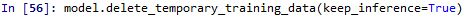
\includegraphics[scale=0.7]{figures/1174009/chapter5/49.jpg}
\caption{Model Disave dan Temporari Train Hapus}
\label{Model Disave dan Temporari Train Hapus}
\end{figure}

\begin{figure}[!hbtp]
\centering
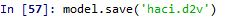
\includegraphics[scale=0.7]{figures/1174009/chapter5/50.jpg}
\caption{Model Disave dan Temporari Train Hapus}
\label{Model Disave dan Temporari Train Hapus}
\end{figure}

Penjelasan:

Untuk mencegah ram agar tidak lemot atau lambat. Sedangkan kenapa temporari training harus dihapus mengosongkan memori agar sedikit lega atau tidak lemot.

\end{itemize}

\item Infercode
\begin{itemize}
\item Contoh atau Ilustrasi Gambar:

\begin{figure}[!hbtp]
\centering
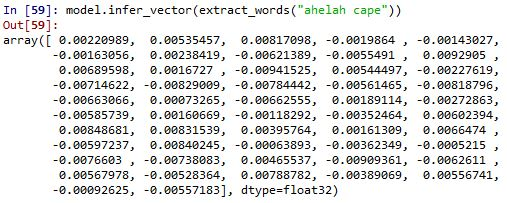
\includegraphics[scale=0.7]{figures/1174009/chapter5/51.jpg}
\caption{Infercode}
\label{Infercode}
\end{figure}

Penjelasan:

Untuk menyimpulkan vektor yang berhubungan dengan vektor dokumen baru dan output tersebut merupakan sebuah array.

\end{itemize}

\item Cosinesimilarity
\begin{itemize}
\item Contoh atau Ilustrasi Gambar:

\begin{figure}[!hbtp]
\centering
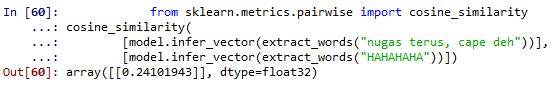
\includegraphics[scale=0.7]{figures/1174009/chapter5/52.jpg}
\caption{Cosinesimilarity}
\label{Cosinesimilarity}
\end{figure}

\begin{figure}[!hbtp]
\centering
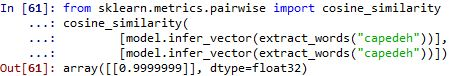
\includegraphics[scale=0.7]{figures/1174009/chapter5/53.jpg}
\caption{Cosinesimilarity}
\label{Cosinesimilarity}
\end{figure}

\begin{figure}[!hbtp]
\centering
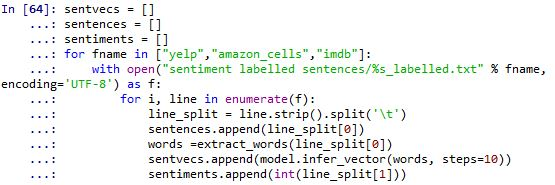
\includegraphics[scale=0.7]{figures/1174009/chapter5/54.jpg}
\caption{Cosinesimilarity}
\label{Cosinesimilarity}
\end{figure}

\begin{figure}[!hbtp]
\centering
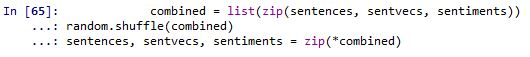
\includegraphics[scale=0.7]{figures/1174009/chapter5/55.jpg}
\caption{Cosinesimilarity}
\label{Cosinesimilarity}
\end{figure}

Penjelasan: 

Cosine Similarity dapat diimplementasikan untuk menghitung nilai kemiripan antar kalimat dan menjadi salah satu teknik untuk mengukur kemiripan  teks yang  popular. 

\end{itemize}

\item Praktek Score Dari Cross Validation
\begin{itemize}
\item Contoh atau Ilustrasi Gambar:

\begin{figure}[!hbtp]
\centering
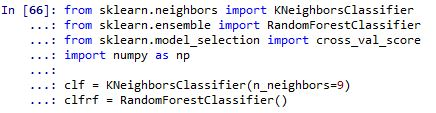
\includegraphics[scale=0.7]{figures/1174009/chapter5/56.jpg}
\caption{Score Cross Validation}
\label{Score Cross Validation}
\end{figure}

\begin{figure}[!hbtp]
\centering
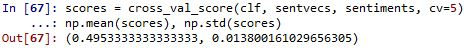
\includegraphics[scale=0.7]{figures/1174009/chapter5/57.jpg}
\caption{Score Cross Validation}
\label{Score Cross Validation}
\end{figure}

\begin{figure}[!hbtp]
\centering
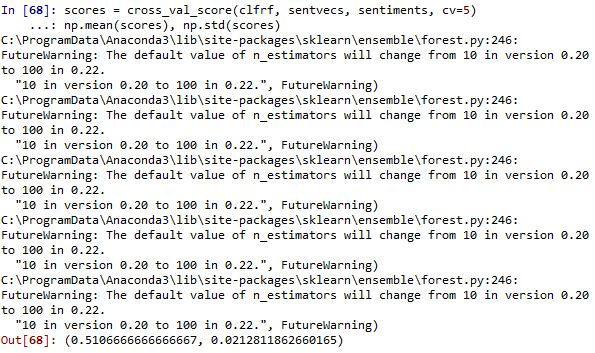
\includegraphics[scale=0.7]{figures/1174009/chapter5/58.jpg}
\caption{Score Cross Validation}
\label{Score Cross Validation}
\end{figure}

\begin{figure}[!hbtp]
\centering
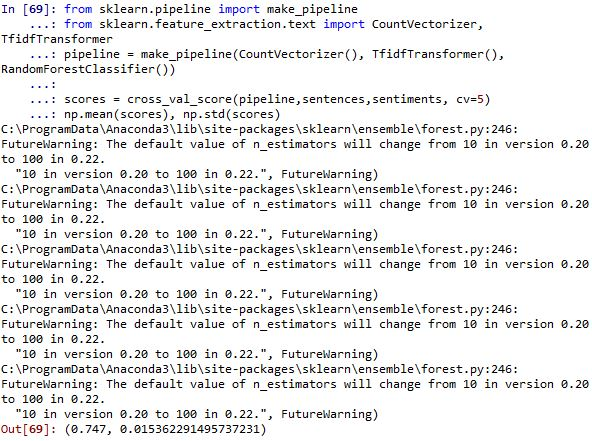
\includegraphics[scale=0.7]{figures/1174009/chapter5/59.jpg}
\caption{Score Cross Validation}
\label{Score Cross Validation}
\end{figure}

Penjelasan: 

Hasil dari praktek tersebut menunjukan untuk menghitung memprediksi dan mengetahui keakuratan dari suatu nilai.

\item PENANGANAN ERROR
\begin{itemize}
\item Contoh atau Ilustrasi Gambar:

\begin{figure}[!hbtp]
\centering
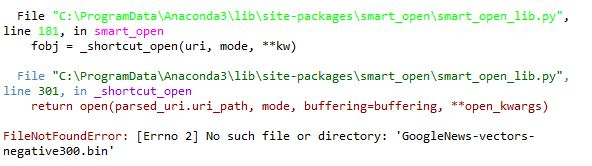
\includegraphics[scale=0.7]{figures/1174009/chapter5/11Error.jpg}
\caption{Error}
\label{Error}
\end{figure}

Solusi:

Pastikan dataset berada dalam satu folder.

\end{itemize}
\end{itemize}
\end{enumerate}